\documentclass{ximera}

\usepackage{epsfig}

\graphicspath{
  {./}
  {figures/}
}


\usepackage{morewrites}

%\newcounter{ccounter}
%\setcounter{ccounter}{1}
%\newcommand{\Chapter}[1]{\setcounter{chapter}{\arabic{ccounter}}\chapter{#1}\addtocounter{ccounter}{1}}

%\newcommand{\section}[1]{\section{#1}\setcounter{thm}{0}\setcounter{equation}{0}}

%\renewcommand{\theequation}{\arabic{chapter}.\arabic{section}.\arabic{equation}}
%\renewcommand{\thefigure}{\arabic{chapter}.\arabic{figure}}
%\renewcommand{\thetable}{\arabic{chapter}.\arabic{table}}

%\newcommand{\Sec}[2]{\section{#1}\markright{\arabic{ccounter}.\arabic{section}.#2}\setcounter{equation}{0}\setcounter{thm}{0}\setcounter{figure}{0}}

\newcommand{\Sec}[2]{\section{#1}}

\setcounter{secnumdepth}{2}
%\setcounter{secnumdepth}{1} 

%\newcounter{THM}
%\renewcommand{\theTHM}{\arabic{chapter}.\arabic{section}}

\newcommand{\trademark}{{R\!\!\!\!\!\bigcirc}}
%\newtheorem{exercise}{}

\newcommand{\dfield}{{\sf dfield9}}
\newcommand{\pplane}{{\sf pplane9}}

\newcommand{\EXER}{\section*{Exercises}}%\vspace*{0.2in}\hrule\small\setcounter{exercise}{0}}
\newcommand{\CEXER}{}%\vspace{0.08in}\begin{center}Computer Exercises\end{center}}
\newcommand{\TEXER}{} %\vspace{0.08in}\begin{center}Hand Exercises\end{center}}
\newcommand{\AEXER}{} %\vspace{0.08in}\begin{center}Hand Exercises\end{center}}

% BADBAD: \newcommand{\Bbb}{\bf}

\newcommand{\R}{\mbox{$\Bbb{R}$}}
\newcommand{\C}{\mbox{$\Bbb{C}$}}
\newcommand{\Z}{\mbox{$\Bbb{Z}$}}
\newcommand{\N}{\mbox{$\Bbb{N}$}}
\newcommand{\D}{\mbox{{\bf D}}}
\usepackage{amssymb}
%\newcommand{\qed}{\hfill\mbox{\raggedright$\square$} \vspace{1ex}}
%\newcommand{\proof}{\noindent {\bf Proof:} \hspace{0.1in}}

\newcommand{\setmin}{\;\mbox{--}\;}
\newcommand{\Matlab}{{M\small{AT\-LAB}} }
\newcommand{\Matlabp}{{M\small{AT\-LAB}}}
\newcommand{\computer}{\Matlab Instructions}
\newcommand{\half}{\mbox{$\frac{1}{2}$}}
\newcommand{\compose}{\raisebox{.15ex}{\mbox{{\scriptsize$\circ$}}}}
\newcommand{\AND}{\quad\mbox{and}\quad}
\newcommand{\vect}[2]{\left(\begin{array}{c} #1_1 \\ \vdots \\
 #1_{#2}\end{array}\right)}
\newcommand{\mattwo}[4]{\left(\begin{array}{rr} #1 & #2\\ #3
&#4\end{array}\right)}
\newcommand{\mattwoc}[4]{\left(\begin{array}{cc} #1 & #2\\ #3
&#4\end{array}\right)}
\newcommand{\vectwo}[2]{\left(\begin{array}{r} #1 \\ #2\end{array}\right)}
\newcommand{\vectwoc}[2]{\left(\begin{array}{c} #1 \\ #2\end{array}\right)}



\newcommand{\inv}{^{-1}}
\newcommand{\CC}{{\cal C}}
\newcommand{\CCone}{\CC^1}
\newcommand{\Span}{{\rm span}}
\newcommand{\rank}{{\rm rank}}
\newcommand{\trace}{{\rm tr}}
\newcommand{\RE}{{\rm Re}}
\newcommand{\IM}{{\rm Im}}
\newcommand{\nulls}{{\rm null\;space}}

\newcommand{\dps}{\displaystyle}
\newcommand{\arraystart}{\renewcommand{\arraystretch}{1.8}}
\newcommand{\arrayfinish}{\renewcommand{\arraystretch}{1.2}}
\newcommand{\Start}[1]{\vspace{0.08in}\noindent {\bf Section~\ref{#1}}}
\newcommand{\exer}[1]{\noindent {\bf \ref{#1}}}
\newcommand{\ans}{}
\newcommand{\matthree}[9]{\left(\begin{array}{rrr} #1 & #2 & #3 \\ #4 & #5 & #6
\\ #7 & #8 & #9\end{array}\right)}
\newcommand{\cvectwo}[2]{\left(\begin{array}{c} #1 \\ #2\end{array}\right)}
\newcommand{\cmatthree}[9]{\left(\begin{array}{ccc} #1 & #2 & #3 \\ #4 & #5 &
#6 \\ #7 & #8 & #9\end{array}\right)}
\newcommand{\vecthree}[3]{\left(\begin{array}{r} #1 \\ #2 \\
#3\end{array}\right)}
\newcommand{\cvecthree}[3]{\left(\begin{array}{c} #1 \\ #2 \\
#3\end{array}\right)}
\newcommand{\cmattwo}[4]{\left(\begin{array}{cc} #1 & #2\\ #3
&#4\end{array}\right)}

\newcommand{\Matrix}[1]{\ensuremath{\left(\begin{array}{rrrrrrrrrrrrrrrrrr} #1 \end{array}\right)}}

\newcommand{\Matrixc}[1]{\ensuremath{\left(\begin{array}{cccccccccccc} #1 \end{array}\right)}}



\renewcommand{\labelenumi}{\theenumi)}
\newenvironment{enumeratea}%
{\begingroup
 \renewcommand{\theenumi}{\alph{enumi}}
 \renewcommand{\labelenumi}{(\theenumi)}
 \begin{enumerate}}
 {\end{enumerate}\endgroup}



\newcounter{help}
\renewcommand{\thehelp}{\thesection.\arabic{equation}}

%\newenvironment{equation*}%
%{\renewcommand\endequation{\eqno (\theequation)* $$}%
%   \begin{equation}}%
%   {\end{equation}\renewcommand\endequation{\eqno \@eqnnum
%$$\global\@ignoretrue}}

%\input{psfig.tex}

\author{Martin Golubitsky and Michael Dellnitz}

%\newenvironment{matlabEquation}%
%{\renewcommand\endequation{\eqno (\theequation*) $$}%
%   \begin{equation}}%
%   {\end{equation}\renewcommand\endequation{\eqno \@eqnnum
% $$\global\@ignoretrue}}

\newcommand{\soln}{\textbf{Solution:} }
\newcommand{\exercap}[1]{\centerline{Figure~\ref{#1}}}
\newcommand{\exercaptwo}[1]{\centerline{Figure~\ref{#1}a\hspace{2.1in}
Figure~\ref{#1}b}}
\newcommand{\exercapthree}[1]{\centerline{Figure~\ref{#1}a\hspace{1.2in}
Figure~\ref{#1}b\hspace{1.2in}Figure~\ref{#1}c}}
\newcommand{\para}{\hspace{0.4in}}

\renewenvironment{solution}{\suppress}{\endsuppress}

\ifxake
\newenvironment{matlabEquation}{\begin{equation}}{\end{equation}}
\else
\newenvironment{matlabEquation}%
{\let\oldtheequation\theequation\renewcommand{\theequation}{\oldtheequation*}\begin{equation}}%
  {\end{equation}\let\theequation\oldtheequation}
\fi

\makeatother


\title{Higher Order Equations}

\begin{document}
\begin{abstract}
\end{abstract}
\maketitle


\label{S:RO}

Using the same trick as in the case of equations with constant 
coefficients we can rewrite a higher order linear equation with
nonconstant coefficients as a first order system of linear
equations.  This way we can also use the method of variation 
of parameters for the solution of higher order equations.  
In fact, consider a general linear differential equation of 
order\index{order} $n$
\begin{equation}
\label{E:noncc}
\frac{d^nx}{dt^n} + a_{n-1}(t)\frac{d^{n-1}x}{dt^{n-1}} +\cdots + 
a_1(t)\frac{dx}{dt}+a_0(t)x = g(t).
\end{equation}\index{differential equation!higher order}
As in Section~\ref{sec:HighOrder} we define the functions
$x_1(t),\ldots,x_n(t)$ by
\[
x_1(t)=x(t),\quad x_2(t)=\frac{dx}{dt}(t),\quad
\ldots, \quad  x_n(t)=\frac{d^{n-1}x}{dt^{n-1}}(t)
\]
and see that \eqref{E:noncc} is equivalent to
\arraystart
\[
\begin{array}{rcl}
\dps \frac{dx_j}{dt}&=&x_{j+1} \hspace{1.6in} (j=1,\ldots,n-1)\\
\dps \frac{dx_n}{dt}&=& g(t) - a_0(t)x_1 - \cdots - a_{n-1}(t) x_n.
\end{array}
\]
\arrayfinish
Introducing the vectors
\[
X(t) = (x_1(t),\ldots,x_n(t))^t  \AND
G(t) = (0,\ldots,0,g(t))^t
\]
we conclude that \eqref{E:noncc} is equivalent to the 
first order system\index{first order!reduction to}
\[
\frac{dX}{dt} = A(t)X+G(t),
\]
where $A(t)$ is the matrix
\[
A(t) = \left(\begin{array}{ccccc}
0 & 1 & 0 & \cdots & 0\\
0 & 0 & 1 & \cdots & 0\\
\vdots & \vdots & \vdots & & \vdots\\
0 & 0 & 0 & \cdots & 1\\
-a_0(t) & -a_1(t) &  -a_2(t) & \cdots & -a_{n-1}(t)
\end{array}\right).
\]
In particular, $x_1(t)$ is a solution of \eqref{E:noncc} if 
$X(t)=(x_1(t),\ldots,x_n(t))^t$ is a solution of the system
$\dot X = A(t)X+G(t)$ which can in principle be solved by
variation of parameters.

\subsubsection*{An Example of Second Order}

As an example we find a solution to the initial value
problem 
\begin{equation}
\label{E:2ndorderex}
\begin{array}{c}
\dps \ddot x - \frac{2}{t} \dot x + \frac{2}{t^2} x = t,\\
\dps x(1) = 0,\quad \dot x(1) = 1.
\end{array}
\end{equation}
This second order differential equation is equivalent to the system
\begin{equation}  \label{E:2ndexam}
\begin{array}{rcl}
\dps \dot{X} & = & A(t) X + G(t) \\
\dps X(1) & = & (0,1)^t,
\end{array}
\end{equation}
where 
\[
A(t) = \mattwo{0}{1}{-\frac{2}{t^2}}{\frac{2}{t}}\AND G(t) = \vectwo{0}{t}.
\]

\paragraph{Step 1:}  A basis of solutions\index{basis!of solutions} 
to the homogeneous equation $\dot X = A(t)X$ is
\[
X_1(t) = \vectwo{t}{1} \AND X_2(t) = \vectwo{t^2}{2t}.
\]

\paragraph{Step 2:}  The inverse of $Y(t)$ is given by
\[
Y(t)^{-1} = \frac{1}{t^2} \mattwo{2t}{-t^2}{-1}{t}.
\]
Hence we obtain
\[
D(t) = Y(t)^{-1} G(t) = \frac{1}{t^2} \mattwo{2t}{-t^2}{-1}{t}\vectwo{0}{t}  
= \vectwo{-t}{1}
\]

\paragraph{Step 3:} Note that 
\[
X(1) = \vectwo{0}{1} = c_1(1)\vectwo{1}{1} + c_2(1)\vectwo{1}{2}.
\]
So $c_1(1)=-1$ and $c_2(1)=1$.  Now solve the differential equations
\[
\begin{array}{rclcl}
\dot{c}_1 & = & d_1(t) & = & -t \\
\dot{c}_2 & = & d_2(t) & = & 1,
\end{array}
\]
with these initial conditions obtaining
\begin{eqnarray*}
c_1(t) & = & -\frac{1}{2}(t^2+1) \\
c_2(t) & = & t.
\end{eqnarray*}

\paragraph{Step 4:}  Theorem~\ref{thm:varparsys} implies that the 
solution to \eqref{E:2ndexam} is
\[
X(t) = c_1(t)X_1(t) + c_2(t)X_2(t) = \left(\begin{array}{c}
\frac{t}{2}(t^2-1)\\ \frac{1}{2}(3t^2-1) \end{array}\right),
\]
and hence the solution of \eqref{E:2ndorderex} is given by
\[
x(t) = \frac{t}{2}(t^2-1).
\]

\subsubsection*{An Example of an Electrical Circuit}
\index{RLC circuit}\index{electrical circuit}

It is rare, however, that variation of parameters can actually be 
used to find a closed form solution\index{closed form solution} 
to an inhomogeneous higher order 
linear differential equations with variable coefficients.  In such 
instances it is best to resort to numerical integration of the first 
order system obtained from the higher order equation.   

We consider here the temporal behavior of an RLC-circuit introduced in 
Section~\ref{S:SOFE}.  This circuit is described by the differential equation
\[
\ddot x + \frac{R}{L}\dot x +
\frac{1}{CL}x = \frac{1}{CL}V(t),
\]
where $x(t)$ is the voltage drop at the capacitor,
\index{capacitor}\index{resistor}\index{coil}
$R$ is the resistance, $L$ is the inductance,
$C$ is the capacitance, and a voltage source\index{voltage source} 
is producing a time 
dependent voltage $V(t)$, see \eqref{e:eleccirc} in Chapter~\ref{C:LT}.
Now we assume that the circuit additionally
contains a microphone\index{microphone} that has a time dependent 
resistance $R_{mic}(t)$ of the form
\[
R_{mic}(t) = R_0 + R_1\cos(\omega t).
\]
This corresponds to the fact that a periodic signal of 
frequency\index{frequency} 
$\frac{2\pi}{\omega}$ is entering the microphone.  Then
the differential equation for the electrical circuit becomes
\begin{equation}
\label{E:RCLMcir}
\ddot x + \frac{R+R_{mic}(t)}{L}\dot x +
\frac{1}{CL}x = \frac{1}{CL}V(t).
\end{equation}
For simplicity we set
\[
R=0 \AND C=L=R_0 = R_1 = \omega = 1
\]
and assume that the voltage source is producing the constant voltage
\[
V(t) = 1.
\]
Thus we obtain the following linear differential equation of second order
\[
\ddot x + (1+\cos t)\dot x + x = 1,
\]
which is equivalent to the system $\dot X= A(t)X + G(t)$, where
\begin{matlabEquation} \label{E:RCLM}
A(t) = \left( \begin{array}{cc}0 & 1\\-1 & -(1+\cos t)\end{array}\right)
\AND G(t) = \vectwo{0}{1}.
\end{matlabEquation}
It is not obvious how to find the general solution\index{general solution} 
of this equation by hand.
In fact, it is not even clear how to construct solutions of the
homogeneous equation.  Hence we have to rely on numerical methods
and compute solutions using {\tt ode45}\index{\computer!ode45} 
in \Matlabp.  The right hand
side in \eqref{E:RCLM} is stored in the function m-file {\tt f17\_4\_5.m}.
For completeness,
\begin{verbatim}
function f = f17_4_5(t,x)
A = [0  1; -1  -(1+cos(t))];
f = A*x + [0; 1];
\end{verbatim}
We compute the solution of \eqref{E:RCLM} with initial condition $X(0)=(1,1)^t$
for $t\in[0,30]$ by typing
\begin{verbatim}
[t,x] = ode45('f17_4_5',[0 30],[1,1]');
\end{verbatim}
The result of this computation is shown in Figure~\ref{Fig:micro1}.
\begin{figure*}[htb]
 \centerline{%
           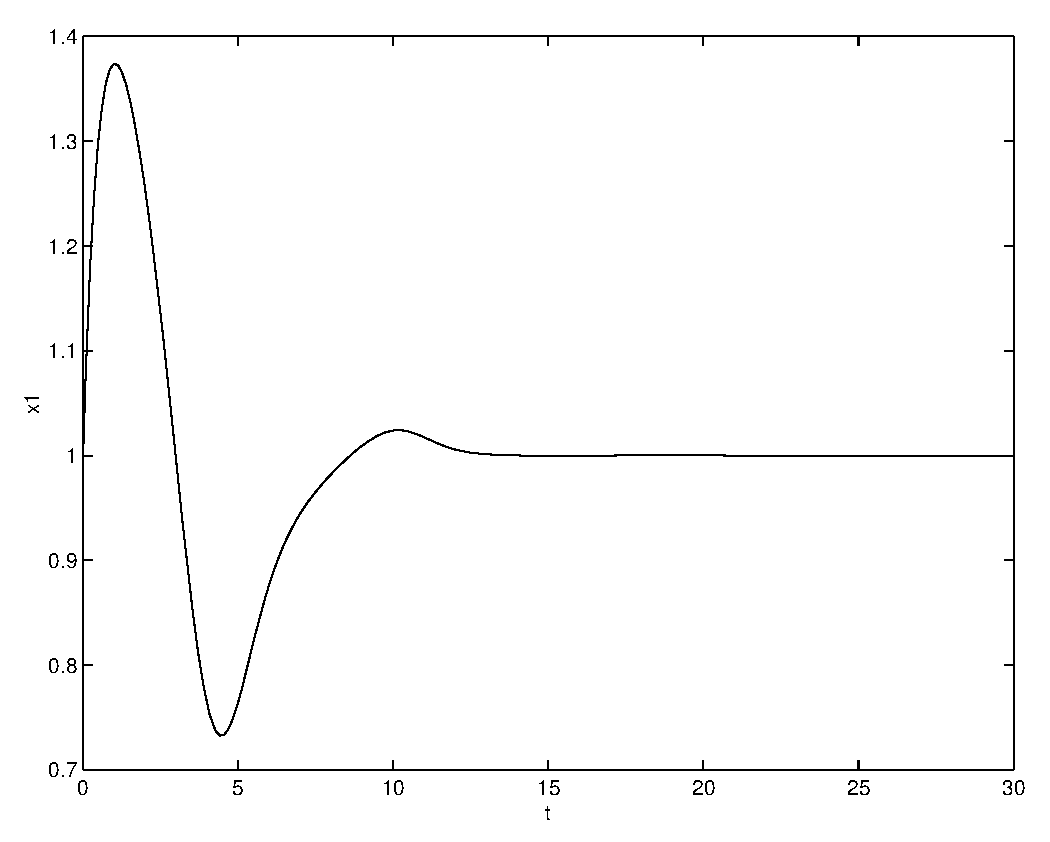
\psfig{file=../figures/microx1.eps,width=3.0in}
	   \psfig{file=../figures/microx2.eps,width=3.0in}}
           \caption{The two components of the solution of 
	   \protect\eqref{E:RCLM} for $t\in[0,30]$ with initial
	   condition $X(0)=(1,1)^t$.}
           \label{Fig:micro1}
\end{figure*}
It can be observed that $x_1(t)$ tends to $1$ and $x_2(t)$ tends to
$0$ for increasing time $t$.  In other words, the solution approaches the 
time independent solution $X(t)=(1,0)^t$ of \eqref{E:RCLM}.

\subsection*{Reduction of Order}
\index{reduction of order}

In order to find solutions to a higher order linear differential equation 
we have rewritten the higher order equation as a first order
system of linear equations, and then we applied variation of
parameters to that system.  There is another method known as
{\em reduction of order\/} that uses the same idea for the
construction principle of the solution --- but this idea is applied directly 
to the higher order equation.  We remark that {\em reduction of
order\/} can sometimes work even when a method like undetermined 
coefficients fails, since its applicability does not depend on the 
specific type of the inhomogeneity.  However, as in the case 
of variation of parameters, the practical use of this technique is very 
limited.  The reason is that the integrations that are involved in the 
computations can rarely be performed by hand.


We illustrate this method by the second order linear differential 
equation
\begin{equation}  \label{e:inhom2}
\ddot{x} + a_1(t)\dot{x} + a_0(t)x = g(t).
\end{equation}
Roughly speaking, reduction of order is a way to reduce the second order 
inhomogeneous equation to an inhomogeneous first order equation.

Suppose that $x_h(t)$ is a solution of the 
homogeneous\index{homogeneous} second order equation
$\ddot{x} + a_1(t)\dot{x} + a_0(t)x = 0$.  
In analogy to the method of variation of
parameters, we try to find a solution $x(t)$ of the 
inhomogeneous\index{inhomogeneous} equation
\eqref{e:inhom2} of the form
\[
x(t) = c(t) x_h(t),
\]
where $c(t)$ is a smooth function.  To determine $c(t)$ we substitute $x(t)$
into the inhomogeneous equation \eqref{e:inhom2}.  Before proceeding, we
compute the derivatives of $x(t)$:
\begin{eqnarray*}
\dot x  & = & \dot c x_h + c \dot{x}_h,\\
\ddot x & = & \ddot c x_h + 2 \dot c \dot{x}_h + c \ddot{x}_h.
\end{eqnarray*}
Next, we substitute $\dot{x}$ and $\ddot{x}$ into \eqref{e:inhom2} and find
\begin{eqnarray*}
&& \ddot c x_h +2\dot c \dot{x}_h + c \ddot{x}_h +
a_1(t)\left(\dot c x_h + c \dot{x}_h \right)+ a_0(t) c x_h =\\
&& x_h \left(\ddot c + \dot c(2 \frac{\dot{x}_h}{x_h} + a_1(t))\right) +
 c(\ddot{x}_h +a_1(t) \dot{x}_h +a_0(t) x_h) = g(t).
\end{eqnarray*}
Since $x_h$ is a solution of the homogeneous equation we have that
$\ddot{x}_h +a_1(t) \dot{x}_h +a_0(t)x_h=0$. After dividing by $x_h$ the function
$c(t)$ satisfies
\[
\ddot c + \dot c\left( 2\frac{\dot{x}_h}{x_h} +a_1(t)\right) = \frac{g(t)}{x_h}.
\]
Introducing $y(t)=\dot c(t)$, we arrive at the differential equation
\[
\frac{dy}{dt} = -y\left( 2\frac{\dot{x}_h}{x_h} +a_1(t)\right) + \frac{g(t)}{x_h}
\]
which is linear and of first order.  If we can find a solution
$y(t)$ of this equation then we can compute $c(t)$ by integration
and we have constructed a 
particular solution\index{reduction of order!particular solution} 
$x(t)=c(t)x_h(t)$ of the
inhomogeneous equation \eqref{e:inhom2}. Thus
\begin{theorem}[Reduction of Order]  \label{thm:redord}
Consider the inhomogeneous linear ODE of second order \eqref{e:inhom2}.
\begin{itemize}
\item[(a)] Let $x_h(t)$ be a nonzero solution of the homogeneous equation
\[
\ddot{x} + a_1(t)\dot{x} + a_0(t)x = 0.
\]
\item[(b)] Let $c(t)$ be a function such that its derivative 
$\dot c(t)$ is a solution of the linear differential equation
\begin{equation}  \label{eq:ro}
\frac{dy}{dt} = -\left(\frac{2\dot x_h(t)+a_1(t) x_h(t)}{x_h(t)}\right)y
+\frac{g(t)}{x_h(t)}.
\end{equation}
\end{itemize}
Then $x_p(t)=c(t) x_h(t)$ is a particular 
solution\index{reduction of order!particular solution} of the second
order inhomogeneous equation \eqref{e:inhom2}.
\end{theorem}\index{reduction of order}

Observe that \eqref{eq:ro} is again a scalar first order differential
equation that can in principle be solved by variation of 
parameters\index{variation of parameters} (see Theorem~\ref{thm:varpar}).
Indeed, to see this one has to substitute
\[
 -\left(\frac{2\dot x_h(t)+a_1(t) x_h(t)}{x_h(t)}\right)
\AND \frac{g(t)}{x_h(t)}.
\]
for
\[
a(t) \AND g(t)
\]
in \eqref{eq:linode1}.




\subsubsection*{A Specific Case: Constant Coefficients and Real Eigenvalues}

As a special case of Theorem~\ref{thm:redord}, we suppose that 
the coefficients $a_0$ and $a_1$ do not depend on $t$ and that $\lambda$ is a
real root of the characteristic 
polynomial\index{characteristic polynomial!of higher order ODE} 
of the homogeneous equation
$\ddot{x} + a_1\dot{x} + a_0x = 0$.  Then we can choose $x_h(t)=e^{\lambda t}$
and \eqref{eq:ro} becomes
\begin{equation}  \label{eq:redeqreal}
\frac{dy}{dt} = -(2\lambda +a_1) y + e^{-\lambda t}g(t).
\end{equation}
If $\dot c(t)$ is a solution to \eqref{eq:redeqreal}, then
$x(t)=c(t) e^{\lambda t}$ is a particular 
solution\index{reduction of order!particular solution} 
of the second order inhomogeneous equation \eqref{e:inhom2}.

As an example, apply reduction of order to find a solution to the inhomogeneous
ODE
\begin{equation}  \label{e:inhomex1}
\ddot{x} - 2\dot{x} + x = \frac{e^t}{t^3}.
\end{equation}
Observe that this equation cannot be solved by the method of undetermined
coefficients\index{undetermined coefficients} since the right hand 
side in \eqref{e:inhomex1} is not a
solution of a homogeneous linear differential equation with constant 
coefficients.

The characteristic polynomial of \eqref{e:inhomex1} has the double eigenvalue 
$\lambda = 1$.  Since $a_1=-2$ and $g(t) = e^t/t^3$, \eqref{eq:redeqreal} takes 
the form
\[
\frac{dy}{dt} = -(2\lambda -2) y + e^{-\lambda t}\left( \frac{e^t}{t^3}\right)
= \frac{1}{t^3}.
\]
Hence 
\[
y(t) = -\frac{1}{2t^2}
\]
and integrating $y(t)$ leads to
\[
c(t) = \int y(t) dt = \frac{1}{2t}.
\]
Now Theorem~\ref{thm:redord} guarantees that
\[
x(t) = c(t)e^t = \frac{e^t}{2t}
\]
is a solution to \eqref{e:inhomex1}.  The other solutions to the inhomogeneous
equation are found by adding the general solution\index{general solution} 
to the homogeneous equation.



\EXER

\TEXER

\noindent In Exercises~\ref{c14.3.2a} -- \ref{c14.3.2b} transform the given 
second order ODE into a first order system and then solve the initial 
value problem by variation of parameters.

\begin{exercise}  \label{c14.3.2a}
\[
\begin{array}{c}
\dps \ddot x - \frac{6}{t^2} x = 14t^3,\\
\dps x(-1) = -1,\quad \dot x(-1) = 5.
\end{array}
\]
{\bf Hint:} the linearly independent solutions of the homogeneous 
equation are:
\[
x^1_h(t) = t^3,\quad x^2_h(t)=\frac{1}{t^2}.
\]

\begin{solution}
\ans The solution to the initial value problem is 
$x(t) = t^5$.

\soln The second order equation can be written as a system
$\dot{X} = A(t)X + G(t)$, where
\[
A(t) = \mattwo{0}{1}{\frac{6}{t^2}}{0} \AND G(t) = \cvectwo{0}{14t^3}.
\]
We can then solve the system by variation of parameters, as described in
Theorem~\ref{thm:varparsys}:

\paragraph{Step 1.} The hint states that
a basis of solutions to the homogeneous system
$\dot{X} = A(t)X$ is
\[
X_1(t) = \vectwo{t^3}{3t^2} \AND X_2(t) =
\vectwo{\frac{1}{t^2}}{-\frac{2}{t^3}}.
\]
\paragraph{Step 2.} To compute the vector $D(t)$, first compute
\[
Y(t)^{-1} = (X_1(t)|X_2(t))^{-1} =
\cmattwo{t^3}{\frac{1}{t^2}}{3t^2}{-\frac{2}{t^3}}^{-1} =
\frac{1}{5}\cmattwo{\frac{2}{t^3}}{\frac{1}{t^2}}{3t^2}{-t^3}.
\]
Then,
\[
D(t) = Y(t)^{-1}G(t) =
\frac{14}{5}\cvectwo{t}{-t^6}.
\]
\paragraph{Step 3.} We find $c_1(-1)$ and $c_2(-1)$ using the initial
condition
\[
X_0 = c_1(-1)X_1(-1) + c_2(-1)X_2(-1).
\]
Therefore,
\[
\vectwo{-1}{5} = c_1(-1)\vectwo{-1}{3} + c_2(-1)\vectwo{1}{2}.
\]
Solve this system to obtain $c_1(-1) = 1.4$ and $c_2(-1) = 0.4$.  By
definition,
$\dot{c_j} = d_j$.  Thus,
\[
c_1(t) = \int_{t_0}^td_1(\tau)d\tau + c_1(-1)
= \frac{14}{5}\int_{-1}^t\tau d\tau + 1.4 = \frac{7}{5}t^2.
\]
\[
c_2(t) = \int_{t_0}^td_2(\tau)d\tau + c_2(-1)
= -\frac{14}{5}\int_{-1}^t\tau^6 d\tau + 0.4= -\frac{2}{5}t^7.
\]
\paragraph{Step 4.} So, the solution to the initial value problem is
\[
X(t) = c_1(t)X_1(t) + c_2(t)X_2(t) = \cvectwo{t^5}{5t^4},
\]
and the first component is the solution to the given second order
equation.


\end{solution}
\end{exercise}

\begin{exercise}  \label{c14.3.2b}
\[
\begin{array}{c}
\dps \ddot x + \frac{2}{t} \dot x - \frac{2}{t^2} x = 4,\\
\dps x(1) = 1,\quad \dot x(1) = 2.
\end{array}
\]
{\bf Hint:} the linearly independent solutions of the homogeneous 
equation are:
\[
x^1_h(t) = t,\quad x^2_h(t)=\frac{1}{t^2}.
\]

\begin{solution}
\ans The solution to the initial value problem is
$x(t) = t^2$.

\soln The second order equation can be written as a system
$\dot{X} = A(t)X + G(t)$, where
\[
A(t) = \mattwo{0}{1}{\frac{2}{t^2}}{-\frac{2}{t}} \AND G(t) = \cvectwo{0}{4}.
\]
We can then solve the system by variation of parameters, as described in
Theorem~\ref{thm:varparsys}:

\paragraph{Step 1.} The hint states that
a basis of solutions to the homogeneous system
$\dot{X} = A(t)X$ is
\[
X_1(t) = \vectwo{t}{1} \AND X_2(t) = \vectwo{\frac{1}{t^2}}{-\frac{2}{t^3}}.
\]
\paragraph{Step 2.} To compute the vector $D(t)$, first compute
\[
Y(t)^{-1} = (X_1(t)|X_2(t))^{-1} =
\cmattwo{t}{\frac{1}{t^2}}{1}{-\frac{2}{t^3}}^{-1} =
\frac{t^2}{3}\cmattwo{\frac{2}{t^3}}{\frac{1}{t^2}}{1}{-t}.
\]
Then,
\[
D(t) = Y(t)^{-1}G(t) = \frac{4}{3}\cvectwo{1}{-t^3}.
\]
\paragraph{Step 3.} We find $c_1(1)$ and $c_2(1)$ using the initial
condition
\[
X_0 = c_1(1)X_1(1) + c_2(1)X_2(1).
\]
Therefore,
\[
\vectwo{1}{2} = c_1(1)\vectwo{1}{1} + c_2(1)\vectwo{1}{-2}.
\]
Solve this system to obtain $c_1(1) = \frac{4}{3}$ and $c_2(1) = -\frac{1}{3}$.
By definition,
$\dot{c_j} = d_j$.  Thus,
\[
c_1(t) = \int_{t_0}^td_1(\tau)d\tau + c_1(1)
= \frac{4}{3}\int_{1}^t 1 d\tau + \frac{4}{3} = \frac{4}{3}t.
\]
\[
c_2(t) = \int_{t_0}^td_2(\tau)d\tau + c_2(1)
= -\frac{4}{3}\int_{1}^t\tau^3 d\tau - \frac{1}{3}= -\frac{t^4}{3}.
\]
\paragraph{Step 4.} So, the solution to the initial value problem is
\[
X(t) = c_1(t)X_1(t) + c_2(t)X_2(t) = \cvectwo{t^2}{2t},
\]
and the first component is the solution to the given second order
equation.

\end{solution}
\end{exercise}

\begin{exercise} \label{c14.3.3}
Use reduction of order to find a solution to the equation
\begin{equation}  \label{e:inhomex2}
\ddot{x} + 3\dot{x}+2x = t.
\end{equation}
Compare the level of effort with the solution obtained using the
method of undetermined coefficients.

\begin{solution}
\ans A particular solution to the equation is given by
$x_p(t) = \frac{1}{2}(t-\frac{3}{2})$.

\soln The roots of the characteristic polynomial of the homogeneous
second order equation $\ddot x + 3\dot x + 2x = 0$
are $\lambda_1 = -1 $ and $\lambda_2 = -2$.
We choose $\lambda_1$ and $x_h(t)=e^{-t}$.  Then we find a solution
$y(t)$ of \eqref{eq:redeqreal}, that is,
\[
\frac{dy}{dt} = -(2\lambda_1 +a_1) y + e^{-\lambda_1 t}g(t) =
-y + te^t.
\]
This can be done by variation of parameters and we apply
Theorem~\ref{thm:varpar}.  Using the notation of this theorem, we can
choose
\[
H(t) = -t \AND c(t) = \int t e^{2t} dt = \frac{1}{2}e^{2t}(t-\frac{1}{2}),
\]
and obtain the solution
\[
y(t) = c(t)e^{H(t)} = \frac{1}{2}e^{t}(t-\frac{1}{2}).
\]
An integration of $y(t)$ now leads to the function $c(t)$ which is needed
for an application of Theorem~\ref{thm:redord}.  We compute
\[
c(t) = \int y(t)dt = \frac{e^t}{2}(t-\frac{3}{2}).
\]
Hence a particular solution is given by
\[
x_p(t) = c(t) x_h(t) =  \frac{1}{2}(t-\frac{3}{2}).
\]
Obviously the level of effort is much greater here than when using the method
of undetermined coefficients.  For a comparison, see the
beginning of Section~\ref{sec:2norderinhom} where
this problem is solved by undetermined coefficients.


\end{solution}
\end{exercise}



\begin{exercise} \label{c14.3.4}
Consider the second order differential equation
\begin{equation}  \label{ex:at1}
\frac{d^2x}{dt^2} + p(t)\frac{dx}{dt} + q(t)x = g(t).
\end{equation}
Suppose that
\[
x_1(t) = 1, \quad  x_2(t) = 1+t, \AND x_3(t) = 1+t+t^2
\]
are all solutions to \eqref{ex:at1}.  Then determine $p(t)$, $q(t)$, and
$g(t)$.

\begin{solution}
\ans $q(t) = \frac{2}{t^2} = g(t)$ and  
$p(t) = -\frac{2}{t}$.

\soln  The three solutions $x_1$, $x_2$, $x_3$ yield three equations
\begin{eqnarray*}
q(t) & = & g(t)\\
p(t) +(1+t)q(t) & = & g(t)\\
2 + (1+2t)p(t) + (1+t+t^2)q(t) & = & g(t).
\end{eqnarray*}
Substituting the $1^{st}$ equation into the $2^{nd}$ equation yields
\[
p(t) + tq(t) = 0.
\]
Therefore, the $3^{rd}$ equation is:
\[
2 - (1+2t)tq(t) + (1+t+t^2)q(t) = 2 + (1-t^2)q(t) = q(t).
\]
Hence 
\[
q(t) = \frac{2}{t^2} = g(t) \AND  p(t) = -\frac{2}{t}.
\]

\end{solution}
\end{exercise}

\begin{exercise} \label{c14.3.4A}
Set $R=0$ and $C=L=1$ in the electrical circuit equation \eqref{E:RCLMcir}. 
Show that this equation may be rewritten as the first order system
\begin{equation} \label{E:ECsy}
\begin{array}{rcl}
\dot{x} & = & y \\
\dot{y} & = & -x -R_{mic}(t)y + V(t).
\end{array} 
\end{equation}

\begin{solution}

With $R=0$ and $C=L=1$, equation \eqref{E:RCLMcir} becomes
\[
\ddot{x} + R_{mic}(t)\dot{x} + x = V(t).
\]
Set $y=\dot{x}$.  Then this equation is
\[
\dot{y} + R_{mic}(t)y + x = V(t).
\]
Solving for $\dot{x}$ and $\dot{y}$ yields the answer. 

\end{solution}
\end{exercise}

\CEXER

\noindent In Exercises~\ref{c14.3.7a} -- \ref{c14.3.7d} use \Matlab
to find solutions for the electrical circuit\index{electrical circuit} 
\eqref{E:RCLMcir}.  In each exercise, set $R=0$ and $C=L=1$ in addition to 
the specified information, and use the first order system \eqref{E:ECsy}.

\begin{exercise} \label{c14.3.7a}
Parameters for the circuit: $R_{mic}(t) = 1+\cos(5t)$ and $V(t) = 1$;\\
initial conditions and time interval: $x(0) = 1$, $\dot{x}(0) = 0.9$ and  
$t\in[0,20]$.

\begin{solution}
\ans The numerically computed solution is displayed in 
Figure~\ref{c14.3.7a}.

\soln  Using the system \eqref{E:ECsy} derived in 
Exercise~\ref{c14.3.4A}, the first order system is:
\begin{eqnarray*}
\dot{x} & = & y \\
\dot{y} & = & -x - (1+\cos(5t))y + 1
\end{eqnarray*}
with initial conditions $x(0)=1$ and $y(0)=0.9$.   To solve this system numerically 
using {\tt ode45}, write the m-file
\begin{verbatim}
function f = ex17_4_6(t,x)
A = [0  1; -1  -(1+cos(5*t))];
f = A*x + [0; 1];
\end{verbatim}
Now solve the differential equation using the command
\begin{verbatim}
[t,x] = ode45('ex17_4_6',[0 20],[1;0.9]);
\end{verbatim}
The solution $x(t)$ may be plotted using the command {\tt plot(t,x(:,1))}; the 
result is displayed in Figure~\ref{c14.3.7a}.
\begin{figure}[htb]
     \centerline{%
     \psfig{file=exfigure/fig17-4-6.eps,width=3.0in}}
        \exercap{c14.3.7a}
\end{figure} 


\end{solution}
\end{exercise}

\begin{exercise} \label{c14.3.7b}
Parameters for the circuit: $R_{mic}(t) = 1+\sin t$ and $V(t) = \sin(2t)$;\\
initial conditions and time interval: $x(0) = 2$, $\dot{x}(0) = 1$ and $t\in[0,40]$.

\begin{solution}
\ans The numerically computed solution is displayed in 
Figure~\ref{c14.3.7b}.

\soln  Using the system \eqref{E:ECsy} derived in 
Exercise~\ref{c14.3.4A}, the first order system is:
\begin{eqnarray*}
\dot{x} & = & y \\
\dot{y} & = & -x - (1+\sin t)y + \sin(2t)
\end{eqnarray*}
with initial conditions $x(0)=2$ and $y(0)=1$.  To solve this system numerically 
using {\tt ode45}, write the m-file
\begin{verbatim}
function f = ex17_4_7(t,x)
A = [0  1; -1  -(1+sin(t))];
f = A*x + [0; sin(2*t)];
\end{verbatim}
Now solve the differential equation using the command
\begin{verbatim}
[t,x] = ode45('ex17_4_7',[0 40],[2;1]);
\end{verbatim}
The solution $x(t)$ may be plotted using the command {\tt plot(t,x(:,1))}; the 
result is displayed in Figure~\ref{c14.3.7b}.
\begin{figure}[htb]
     \centerline{%
     \psfig{file=exfigure/fig17-4-7.eps,width=3.0in}}
        \exercap{c14.3.7b}
\end{figure} 


\end{solution}
\end{exercise}

\begin{exercise} \label{c14.3.7c}
Parameters for the circuit: $R_{mic}(t) = 1+\cos t$ and $V(t) = 0.4+e^{-t}\sin(3t)$;\\
initial conditions and time interval: $x(0) = 1$, $\dot{x}(0) = -1.5$ and 
$t\in[0,30]$.

\begin{solution}
\ans The numerically computed solution is displayed in 
Figure~\ref{c14.3.7c}.

\soln  Using the system \eqref{E:ECsy} derived in 
Exercise~\ref{c14.3.4A}, the first order system is:
\begin{eqnarray*}
\dot{x} & = & y \\
\dot{y} & = & -x - (1+\cos t)y + 0.4 + e^{-t}\sin t
\end{eqnarray*}
with initial conditions $x(0)=1$ and $y(0)=-1.5$. To solve this system numerically 
using {\tt ode45}, write the m-file
\begin{verbatim}
function f = ex17_4_8(t,x)
A = [0  1; -1  -(1+cos(t))];
f = A*x + [0; 0.4+exp(-t)*sin(t)];
\end{verbatim}
Now solve the differential equation using the command
\begin{verbatim}
[t,x] = ode45('ex17_4_8',[0 30],[1;-1.5]);
\end{verbatim}
The solution $x(t)$ may be plotted using the command {\tt plot(t,x(:,1))}; the 
result is displayed in Figure~\ref{c14.3.7c}.
\begin{figure}[htb]
     \centerline{%
     \psfig{file=exfigure/fig17-4-8.eps,width=3.0in}}
        \exercap{c14.3.7c}
\end{figure} 



\end{solution}
\end{exercise}

\begin{exercise} \label{c14.3.7d}
Parameters for the circuit: $R_{mic}(t) = 0.02+\sin t$ and $V(t) = 1$;\\
initial conditions and time interval: $x(0) = 1.2$, $\dot{x}(0) = 1.1$ and 
$t\in[0,60]$.

\begin{solution}
\ans The numerically computed solution is displayed in 
Figure~\ref{c14.3.7d}.

\soln  Using the system \eqref{E:ECsy} derived in 
Exercise~\ref{c14.3.4A}, the first order system is:
\begin{eqnarray*}
\dot{x} & = & y \\
\dot{y} & = & -x - (0.02+\sin t)y + 1
\end{eqnarray*}
with initial conditions $x(0)=1.2$ and $y(0)=1.1$.   To solve this system numerically 
using {\tt ode45}, write the m-file
\begin{verbatim}
function f = ex17_4_9(t,x)
A = [0  1; -1  -(0.02+sin(t))];
f = A*x + [0; 1];
\end{verbatim}
Now solve the differential equation using the command
\begin{verbatim}
[t,x] = ode45('ex17_4_9',[0 60],[1.2;1.1]);
\end{verbatim}
The solution $x(t)$ may be plotted using the command {\tt plot(t,x(:,1))}; the 
result is displayed in Figure~\ref{c14.3.7d}.
\begin{figure}[htb]
     \centerline{%
     \psfig{file=exfigure/fig17-4-9.eps,width=3.0in}}
        \exercap{c14.3.7d}
\end{figure} 





\end{solution}
\end{exercise}



\end{document}
